\chapter{First Release - Core Ingestion and 3D Visualization}

\section{Introduction}
This chapter documents the design, modeling, and realization of the first functional release of the platform, aligning with the \textbf{Release 1} specifications. This release covers \textbf{Sprint 1 (Core Data Ingestion and Scraper Pipeline)} and \textbf{Sprint 2 (Real-Time SSE Streaming and 3D Globe Visualization)}. For each sprint, we present its backlog objectives, UML modeling diagrams (Use Case, Class, and Sequence), database schemas, component structures, code walks, and interface screenshots.

---

\section{Sprint 1: Data Ingestion and Enrichment Pipeline}

\subsection{Sprint Backlog and Objectives}
The core objective of Sprint 1 was to establish the ingestion backend. This included configuring the Express server, setting up Mongoose models, coding the 9 modular scrapers, and implementing the 5-layer sector classification and geolocation enrichment pipeline. 

The primary engineering challenges in this sprint involved managing parallel connections to heterogeneous APIs and transforming varying, unstructured data formats into a unified, compact database schema, ensuring database writes remained performant under high threat volumes.

\subsection{Sprint Analysis: Use Case Modeling}
The ingestion use cases are captured in Figure~\ref{fig:s1_usecase}, illustrating how the External API Feed actor triggers the harvest loop.

\begin{figure}[htbp]
\centering
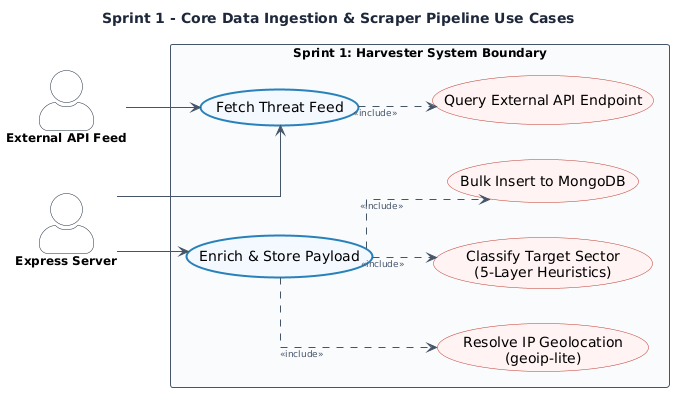
\includegraphics[width=0.95\textwidth]{assets/s1_usecase.png}
\caption{Sprint 1: Use Case diagram for threat data harvesting.}
\label{fig:s1_usecase}
\end{figure}

The functional behaviors of these use cases are structured in Table~\ref{tab:s1_uc_desc}.

\begin{table}[htbp]
\centering
\small
\begin{tabular}{>{\raggedright\arraybackslash}p{3.8cm}>{\raggedright\arraybackslash}p{4.7cm}>{\raggedright\arraybackslash}p{4.7cm}}
\toprule
\textbf{Use Case} & \textbf{Actor/Trigger} & \textbf{Main Workflow} \\
\midrule
Fetch Threat Feed & Express Server (Scheduler / Poll) & The server initiates a scheduler, calling a modular scraper file to query the external REST endpoint or establish a streaming connection, retrieving threat JSON packets. \\
Enrich \& Store Payload & Express Server (Callback / Data In) & Upon retrieval, the payload is resolved through `enrichment.js` for IP geolocation and target sector classification, and queued for bulk MongoDB write. \\
\bottomrule
\end{tabular}
\caption{Sprint 1: Use Case descriptions.}
\label{tab:s1_uc_desc}
\end{table}

\subsection{Sprint Conception: Classes, Sequences, and Schemas}

\subsubsection{UML Class Diagram}
The structural interfaces created in Sprint 1 are illustrated in Figure~\ref{fig:s1_class}.

\begin{figure}[htbp]
\centering
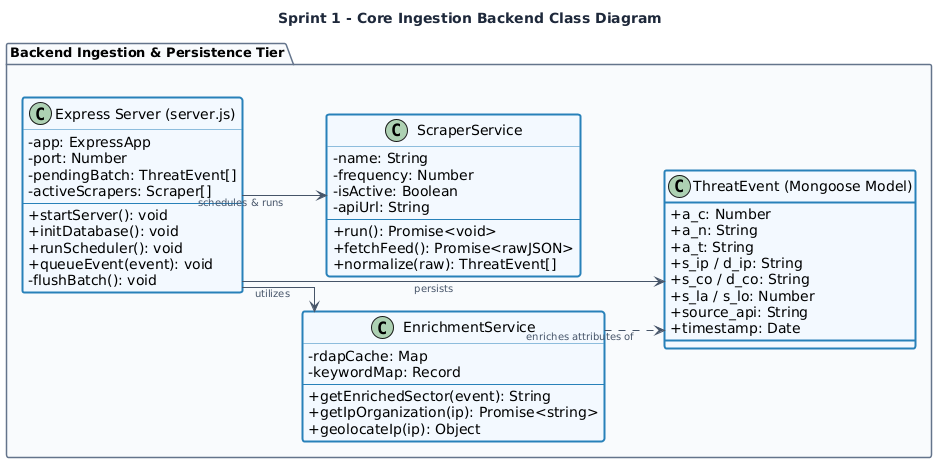
\includegraphics[width=0.95\textwidth]{assets/s1_class.png}
\caption{Sprint 1: Conception Class diagram.}
\label{fig:s1_class}
\end{figure}

\subsubsection{MongoDB Schema Dictionary}
To accommodate high-velocity database writes (up to hundreds of logs per second), the MongoDB schema in `models/ThreatEvent.js` uses \textbf{compact field names} to minimize BSON document sizes. This layout reduces document sizes from 200 bytes to 80 bytes, conserving cloud database storage. Furthermore, a compound index was established on `s\_ip` and `timestamp` to accelerate fast queries on the history explorer page. The database schema dictionary mapping is defined in Table~\ref{tab:db_dictionary}.

\begin{table}[htbp]
\centering
\small
\begin{tabular}{>{\raggedright\arraybackslash}p{3.2cm}>{\raggedright\arraybackslash}p{2.0cm}>{\raggedright\arraybackslash}p{1.4cm}>{\raggedright\arraybackslash}p{6.0cm}}
\toprule
\textbf{BSON Field} & \textbf{Logical Name} & \textbf{Type} & \textbf{Description / Constraints} \\
\midrule
`a\_c` & Attack Count & Number & Aggregated attack volume count (default 1) \\
`a\_n` & Attack Name & String & adversary malware family, CVE identifier, or exploit name \\
`a\_t` & Attack Type & String & Categorized class: `exploit`, `malware`, or `phishing` \\
`s\_ip` / `d\_ip` & Source / Dest IP & String & Resolved IPv4 or IPv6 address \\
`s\_co` / `d\_co` & Source / Dest Country & String & Two-letter ISO country code \\
`s\_la` / `s\_lo` & Source Latitude / Longitude & Number & Geocoded decimal geographic coordinate coordinates \\
`d\_la` / `d\_lo` & Dest Latitude / Longitude & Number & Geocoded target coordinates (or fallback coordinates) \\
`source\_api` & Source Feeds Tag & String & Scraper origin tag (e.g., `alienvault`, `urlhaus`) \\
`timestamp` & Event Timestamp & Date & Date of capture. \textbf{Expires after 30 days (TTL index)} \\
\bottomrule
\end{tabular}
\caption{MongoDB BSON Schema Dictionary (`models/ThreatEvent.js`).}
\label{tab:db_dictionary}
\end{table}

\subsubsection{UML Sequence Diagram}
The transactional messaging timeline tracing threat log polling, geocoding, target enrichment, and bulk database persistence is illustrated in Figure~\ref{fig:s1_sequence}.

\begin{figure}[htbp]
\centering
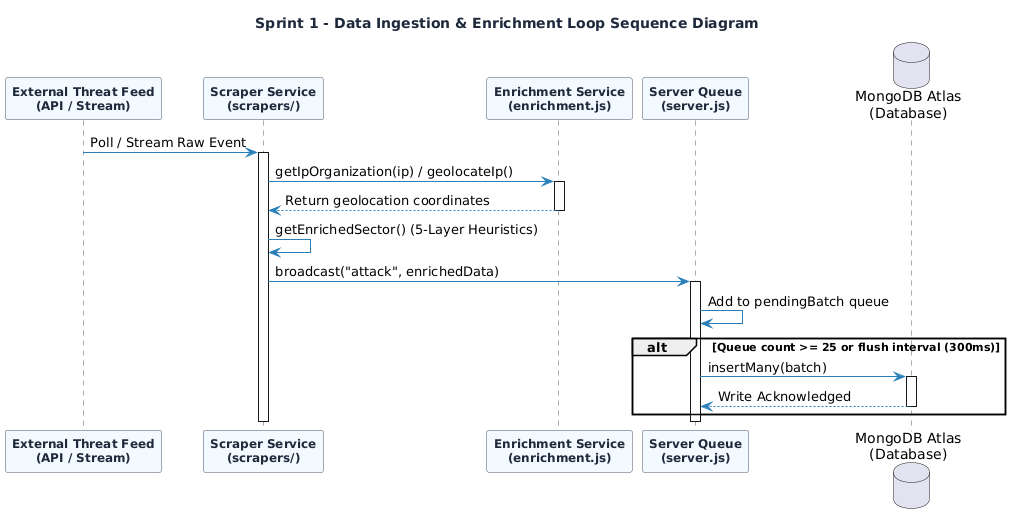
\includegraphics[width=0.95\textwidth]{assets/s1_sequence.png}
\caption{Sprint 1: Sequence diagram of the harvesting and enrichment loop.}
\label{fig:s1_sequence}
\end{figure}

---

\subsection{Sprint Realization: Detailed Scraper Implementations}
The harvesters are located in \texttt{backend/services/scrapers/}. To ensure complete operational isolation, thread resilience, and modular error recovery, we implemented a decoupled execution model. The core Express orchestrator (\texttt{server.js}) dynamically registers each scraper module, executing their ingestion loops within separate asynchronous promise contexts. This ensures that if a single external feed encounters network timeouts, rate-limit blocks, or malformed responses, the remaining scrapers continue to operate.

Below, we catalog and detail the architectural specifications, raw payload schemas, and normalization pipelines for each of the 9 integrated cyber threat intelligence harvesters.

\subsubsection{1. Checkpoint Scraper (\texttt{checkpoint.js})}
\begin{itemize}
    \item \textbf{Source Endpoint \& Protocol:} Establishes a direct, long-lived, secure Server-Sent Events (SSE) HTTP stream connection to Checkpoint's corporate live threat telemetry server (summarized in Table~\ref{tab:spec_checkpoint}).
    \begin{table}[htbp]
    \centering
    \small
    \begin{tabular}{ll}
    \toprule
    \textbf{Specification Parameter} & \textbf{Configuration Value} \\
    \midrule
    Protocol & HTTP/1.1 Server-Sent Events (SSE) \\
    Endpoint URL & \url{https://threatmap.checkpoint.com/feed/live} \\
    Transport Security & TLS 1.3 Encryption \\
    Connection Mode & Active Persistent Client Stream \\
    \bottomrule
    \end{tabular}
    \caption{Checkpoint Scraper Endpoint Specifications.}
    \label{tab:spec_checkpoint}
    \end{table}

    \item \textbf{Expected Payload Schema:} The stream broadcasts newline-separated SSE threat packets. The parsed JSON data attributes are defined in Table~\ref{tab:payload_checkpoint} (with the raw payload example detailed in Appendix I.1).
    \begin{table}[htbp]
    \centering
    \small
    \begin{tabular}{lll}
    \toprule
    \textbf{JSON Attribute} & \textbf{Data Type} & \textbf{Description / Constraints} \\
    \midrule
    \texttt{srcIp} & String & Source IPv4 or IPv6 Address \\
    \texttt{dstIp} & String & Target/Destination IP Address \\
    \texttt{attackName} & String & Exploit name or signature identifier \\
    \texttt{attackType} & String & Threat class category (e.g. \texttt{phishing}) \\
    \texttt{severity} & String & Threat severity level string \\
    \texttt{srcCountry} & String & Origin ISO two-letter country code \\
    \texttt{dstCountry} & String & Target ISO two-letter country code \\
    \bottomrule
    \end{tabular}
    \caption{Checkpoint Raw Threat Payload Schema.}
    \label{tab:payload_checkpoint}
    \end{table}

    \item \textbf{Operation Mechanism:} The scraper operates as an active, persistent client listener. Upon establishing the socket, it parses incoming chunks line-by-line, validating that the packet contains valid \texttt{srcIp} and \texttt{dstIp} parameters.
    \item \textbf{Data Normalization \& Error Handling:} Evaluates incoming event keys and maps them directly into our BSON schema. Phishing indicators are routed to the \texttt{phishing} category. If Checkpoint's stream is disconnected, the module initiates an automated reconnect routine with a 5-second backoff delay, logging a warning to the central controller.
\end{itemize}

\subsubsection{2. Bitdefender Live Telemetry Scraper (\texttt{bitdefender.js})}
\begin{itemize}
    \item \textbf{Source Endpoint \& Protocol:} Establishes a real-time Web Socket connection using the \texttt{socket.io-client} protocol to Bitdefender's global threat intelligence sharing hub (summarized in Table~\ref{tab:spec_bitdefender}).
    \begin{table}[htbp]
    \centering
    \small
    \begin{tabular}{ll}
    \toprule
    \textbf{Specification Parameter} & \textbf{Configuration Value} \\
    \midrule
    Protocol & WebSocket (socket.io Transport) \\
    Endpoint URL & \url{wss://hub.bitdefender.com/threat-telemetry} \\
    Active Channels & 13 Threat Channels (e.g. ransomware, botnet) \\
    Connection Mode & Bidirectional Event Socket \\
    \bottomrule
    \end{tabular}
    \caption{Bitdefender Scraper Endpoint Specifications.}
    \label{tab:spec_bitdefender}
    \end{table}

    \item \textbf{Expected Payload Schema:} The WebSocket channel broadcasts binary frames converted into JSON. The attributes are listed in Table~\ref{tab:payload_bitdefender} (with the raw payload example detailed in Appendix I.2).
    \begin{table}[htbp]
    \centering
    \small
    \begin{tabular}{lll}
    \toprule
    \textbf{JSON Attribute} & \textbf{Data Type} & \textbf{Description / Constraints} \\
    \midrule
    \texttt{event} & String & Event action classifier (e.g. \texttt{detection}) \\
    \texttt{channel} & String & Source channel name mapped to threat vector \\
    \texttt{ip} & String & Intercepted source IP address string \\
    \texttt{country} & String & Origin country code (ISO Alpha-2) \\
    \texttt{malwareName} & String & Specific malware signature family name \\
    \texttt{port} & Number & Target connection port (used for sector mapping) \\
    \bottomrule
    \end{tabular}
    \caption{Bitdefender Raw Threat Payload Schema.}
    \label{tab:payload_bitdefender}
    \end{table}

    \item \textbf{Operation Mechanism:} Subscribes to 13 distinct active channels representing diverse attack vectors (e.g. ransomware, malicious URLs, botnets). The socket interface receives live notifications.
    \item \textbf{Data Normalization:} The channel name determines the target threat class mapping. If the event is received on the \texttt{ransomware} channel, the scraper sets \texttt{a\_t = "malware"} and maps the target sector using port-based heuristics (port 445 maps to "Enterprise Technology").
\end{itemize}

\subsubsection{3. Fortinet FortiGuard Scraper (\texttt{fortinet.js})}
\begin{itemize}
    \item \textbf{Source Endpoint \& Protocol:} Polls Fortinet's active exploit telemetry API using standard stateless HTTP queries (summarized in Table~\ref{tab:spec_fortinet}).
    \begin{table}[htbp]
    \centering
    \small
    \begin{tabular}{ll}
    \toprule
    \textbf{Specification Parameter} & \textbf{Configuration Value} \\
    \midrule
    Protocol & HTTP/1.1 REST API (GET) \\
    Endpoint URL & \url{https://fortiguard.com/api/threats/active} \\
    Custom Headers & \texttt{User-Agent: Predictra-Ingestion-Agent/1.0} \\
    Polling Frequency & Every 4 seconds \\
    \bottomrule
    \end{tabular}
    \caption{Fortinet Scraper Endpoint Specifications.}
    \label{tab:spec_fortinet}
    \end{table}

    \item \textbf{Expected Payload Schema:} The API returns a structured JSON array of exploit records. The schema fields are defined in Table~\ref{tab:payload_fortinet} (with the raw payload example detailed in Appendix I.3).
    \begin{table}[htbp]
    \centering
    \small
    \begin{tabular}{lll}
    \toprule
    \textbf{JSON Attribute} & \textbf{Data Type} & \textbf{Description / Constraints} \\
    \midrule
    \texttt{srcCountry} & String & Full country name of attacker origin \\
    \texttt{dstCountry} & String & Full country name of victim target \\
    \texttt{signatureName} & String & Specific exploit name (e.g. Apache Log4j) \\
    \texttt{attackCount} & Number & Aggregated count of attack occurrences \\
    \texttt{victimSubnet} & String & Masked network subnet of victim \\
    \bottomrule
    \end{tabular}
    \caption{Fortinet Raw Threat Payload Schema.}
    \label{tab:payload_fortinet}
    \end{table}

    \item \textbf{Operation Mechanism:} Evaluates recent active exploit campaigns on a 4-second polling schedule. The scraper iterates through the returned array, parses the country strings into ISO two-letter country codes (e.g. "Germany" to "DE"), and extracts the attack name.
    \item \textbf{Data Normalization:} Since Fortinet records reflect active intrusion attempts, threat events are registered under \texttt{a\_t = "exploit"}, and \texttt{a\_c} is mapped directly to the \texttt{attackCount} parameter.
\end{itemize}

\subsubsection{4. URLhaus Malware Scraper (\texttt{urlhaus.js})}
\begin{itemize}
    \item \textbf{Source Endpoint \& Protocol:} Queries abuse.ch's URLhaus API to retrieve newly identified malicious URL distribution nodes (summarized in Table~\ref{tab:spec_urlhaus}).
    \begin{table}[htbp]
    \centering
    \small
    \begin{tabular}{ll}
    \toprule
    \textbf{Specification Parameter} & \textbf{Configuration Value} \\
    \midrule
    Protocol & HTTP/1.1 REST API (POST) \\
    Endpoint URL & \url{https://urlhaus-api.abuse.ch/v1/urls/recent/} \\
    Polling Frequency & Every 90 seconds \\
    \bottomrule
    \end{tabular}
    \caption{URLhaus Scraper Endpoint Specifications.}
    \label{tab:spec_urlhaus}
    \end{table}

    \item \textbf{Expected Payload Schema:} Returns a dictionary containing a list of active threat URLs. The schema fields for each item are defined in Table~\ref{tab:payload_urlhaus} (with the raw payload example detailed in Appendix I.4).
    \begin{table}[htbp]
    \centering
    \small
    \begin{tabular}{lll}
    \toprule
    \textbf{JSON Attribute} & \textbf{Data Type} & \textbf{Description / Constraints} \\
    \midrule
    \texttt{id} & String & Unique integer identifier for URL block \\
    \texttt{url} & String & Full HTTP/HTTPS address serving malware payload \\
    \texttt{url\_status} & String & Online/offline reachability flag \\
    \texttt{threat} & String & Threat class label (e.g. \texttt{malware\_download}) \\
    \texttt{reporter} & String & Name of threat researcher or bot submitter \\
    \texttt{tags} & Array & Threat signature list tags (e.g. CobaltStrike) \\
    \bottomrule
    \end{tabular}
    \caption{URLhaus Raw Threat Payload Schema.}
    \label{tab:payload_urlhaus}
    \end{table}

    \item \textbf{Operation Mechanism:} The scraper parses the \texttt{urls} list, filtering for entries where \texttt{url\_status} is \texttt{"online"}. It uses regex queries to isolate the IP address or domain name from the raw \texttt{url} string (e.g., extracting \texttt{"185.220.101.5"} as the source IP).
    \item \textbf{Data Normalization:} Since these represent active malware distribution files, all events are registered under \texttt{a\_t = "malware"}. The first entry in the \texttt{tags} array is assigned to \texttt{a\_n}.
\end{itemize}

\subsubsection{5. Kaspersky Feodo Botnet Tracker (\texttt{kaspersky.js})}
\begin{itemize}
    \item \textbf{Source Endpoint \& Protocol:} Polls abuse.ch's Feodo Tracker database of active Botnet command-and-control (C2) servers (summarized in Table~\ref{tab:spec_kaspersky}).
    \begin{table}[htbp]
    \centering
    \small
    \begin{tabular}{ll}
    \toprule
    \textbf{Specification Parameter} & \textbf{Configuration Value} \\
    \midrule
    Protocol & HTTP/1.1 REST (GET) \\
    Endpoint URL & \url{https://feodotracker.abuse.ch/downloads/ipblocklist.csv} \\
    Polling Frequency & Every 60 seconds \\
    \bottomrule
    \end{tabular}
    \caption{Kaspersky Feodo Scraper Endpoint Specifications.}
    \label{tab:spec_kaspersky}
    \end{table}

    \item \textbf{Expected Payload Schema:} The feed returns CSV formatted text lines. The schema fields mapping to the CSV headers are defined in Table~\ref{tab:payload_kaspersky} (with the raw payload example detailed in Appendix I.5).
    \begin{table}[htbp]
    \centering
    \small
    \begin{tabular}{lll}
    \toprule
    \textbf{CSV Attribute} & \textbf{Data Type} & \textbf{Description / Constraints} \\
    \midrule
    \texttt{Firstseen} & Date String & Date/time the node was first registered \\
    \texttt{DstIP} & String & Destination Command \& Control IP address \\
    \texttt{DstPort} & Number & Listening port of the C2 framework \\
    \texttt{Malware} & String & Name of active botnet malware (e.g. Qakbot) \\
    \texttt{Asname} & String & Autonomous System (AS) network ISP name \\
    \bottomrule
    \end{tabular}
    \caption{Kaspersky Feodo Raw Threat Payload Schema.}
    \label{tab:payload_kaspersky}
    \end{table}

    \item \textbf{Operation Mechanism:} The scraper retrieves the CSV string, splits it by newline characters, ignores comment lines, and splits each data line by commas. It extracts the destination IP (\texttt{DstIP}), destination port (\texttt{DstPort}), and the specific malware family (\texttt{Malware}).
    \item \textbf{Data Normalization:} Botnet controller nodes are mapped to \texttt{a\_t = "malware"}. The source IP is assigned to \texttt{DstIP}, and target sectors are mapped based on the listening port (port 443 defaults to "Enterprise Services").
\end{itemize}

\subsubsection{6. AlienVault OTX Pulse Scraper (\texttt{alienvault.js})}
\begin{itemize}
    \item \textbf{Source Endpoint \& Protocol:} Queries the AlienVault Open Threat Exchange REST API, utilizing custom developer API authentication tokens (summarized in Table~\ref{tab:spec_alienvault}).
    \begin{table}[htbp]
    \centering
    \small
    \begin{tabular}{ll}
    \toprule
    \textbf{Specification Parameter} & \textbf{Configuration Value} \\
    \midrule
    Protocol & HTTP/1.1 REST (GET) \\
    Endpoint URL & \url{https://otx.alienvault.com/api/v1/pulses/subscribed} \\
    Custom Headers & \texttt{X-OTX-API-KEY: <custom\_otx\_api\_token>} \\
    Polling Frequency & Every 5 minutes \\
    \bottomrule
    \end{tabular}
    \caption{AlienVault Scraper Endpoint Specifications.}
    \label{tab:spec_alienvault}
    \end{table}

    \item \textbf{Expected Payload Schema:} Returns nested threat pulses. The parsed schema attributes are described in Table~\ref{tab:payload_alienvault} (with the raw payload example detailed in Appendix I.6).
    \begin{table}[htbp]
    \centering
    \small
    \begin{tabular}{lll}
    \toprule
    \textbf{JSON Attribute} & \textbf{Data Type} & \textbf{Description / Constraints} \\
    \midrule
    \texttt{count} & Number & Count of pulse objects returned in response \\
    \texttt{name} & String & Threat intelligence pulse campaign name \\
    \texttt{description} & String & Text summary details of adversary activities \\
    \texttt{indicator} & String & Specific indicator string (IP address or hash) \\
    \texttt{type} & String & IOC type tag indicator (e.g. \texttt{IPv4}, \texttt{FileHash}) \\
    \bottomrule
    \end{tabular}
    \caption{AlienVault Raw Threat Payload Schema.}
    \label{tab:payload_alienvault}
    \end{table}

    \item \textbf{Operation Mechanism:} Polls every 5 minutes, pulling recent indicators of compromise (IOC) from subscribed threat pulses. It parses IP addresses, hashes, and vulnerability details.
    \item \textbf{Data Normalization:} The scraper iterates through the nested \texttt{indicators} array. Only indicators of type \texttt{IPv4} are geolocated. The threat name \texttt{a\_n} is derived from the main pulse \texttt{name}.
\end{itemize}

\subsubsection{7. Ransomwatch Extortion Scraper (\texttt{ransomwatch.js})}
\begin{itemize}
    \item \textbf{Source Endpoint \& Protocol:} Polls the Ransomlook.io API endpoint monitoring active ransomware extortion leak sites (summarized in Table~\ref{tab:spec_ransomwatch}).
    \begin{table}[htbp]
    \centering
    \small
    \begin{tabular}{ll}
    \toprule
    \textbf{Specification Parameter} & \textbf{Configuration Value} \\
    \midrule
    Protocol & HTTP/1.1 REST (GET) \\
    Endpoint URL & \url{https://ransomlook.io/api/posts/recent} \\
    Polling Frequency & Every 10 minutes \\
    \bottomrule
    \end{tabular}
    \caption{Ransomwatch Scraper Endpoint Specifications.}
    \label{tab:spec_ransomwatch}
    \end{table}

    \item \textbf{Expected Payload Schema:} Returns a list of dark web leak site posts. The metadata attributes are defined in Table~\ref{tab:payload_ransomwatch} (with the raw payload example detailed in Appendix I.7).
    \begin{table}[htbp]
    \centering
    \small
    \begin{tabular}{lll}
    \toprule
    \textbf{JSON Attribute} & \textbf{Data Type} & \textbf{Description / Constraints} \\
    \midrule
    \texttt{group} & String & Name of ransomware developer group (e.g. LockBit) \\
    \texttt{post\_title} & String & Title containing victim corporation name string \\
    \texttt{discovered} & Date String & Timestamp when post was first indexed \\
    \texttt{website} & String & Darknet onion address of the extortion site \\
    \bottomrule
    \end{tabular}
    \caption{Ransomwatch Raw Threat Payload Schema.}
    \label{tab:payload_ransomwatch}
    \end{table}

    \item \textbf{Operation Mechanism:} Ransomware attacks target organizations rather than specific IP addresses. When a new post is parsed, the scraper extracts the victim name from \texttt{post\_title} ("Texas Medical Center Inc"). It geolocates the victim based on target location keywords ("Texas" to United States coordinates).
    \item \textbf{Data Normalization:} All events are registered as ransomware indicators under \texttt{a\_t = "malware"}. The target business sector is resolved using our 5-layer classification engine (matching "Medical" to "Healthcare").
\end{itemize}

\subsubsection{8. MontySecurity C2 Tracker (\texttt{c2tracker.js})}
\begin{itemize}
    \item \textbf{Source Endpoint \& Protocol:} Polls the MontySecurity command-and-control tracker endpoint to monitor active listener framework IPs (summarized in Table~\ref{tab:spec_c2tracker}).
    \begin{table}[htbp]
    \centering
    \small
    \begin{tabular}{ll}
    \toprule
    \textbf{Specification Parameter} & \textbf{Configuration Value} \\
    \midrule
    Protocol & HTTP/1.1 REST (GET) \\
    Endpoint URL & \url{https://github.com/c2/active/c2.json} \\
    Polling Frequency & Every 15 minutes \\
    \bottomrule
    \end{tabular}
    \caption{MontySecurity C2 Scraper Endpoint Specifications.}
    \label{tab:spec_c2tracker}
    \end{table}

    \item \textbf{Expected Payload Schema:} Returns active command host framework arrays. The JSON fields are described in Table~\ref{tab:payload_c2tracker} (with the raw payload example detailed in Appendix I.8).
    \begin{table}[htbp]
    \centering
    \small
    \begin{tabular}{lll}
    \toprule
    \textbf{JSON Attribute} & \textbf{Data Type} & \textbf{Description / Constraints} \\
    \midrule
    \texttt{ip} & String & Public IP address of the listening C2 server \\
    \texttt{framework} & String & C2 framework software name (e.g. Cobalt Strike) \\
    \texttt{port} & Number & Server listening port number \\
    \texttt{first\_seen} & String & Date string of initial detection \\
    \bottomrule
    \end{tabular}
    \caption{MontySecurity C2 Raw Threat Payload Schema.}
    \label{tab:payload_c2tracker}
    \end{table}

    \item \textbf{Operation Mechanism:} The scraper parses active C2 servers. The parser extracts host IPs, listening ports, and malware families (e.g. Cobalt Strike, Mythic).
    \item \textbf{Data Normalization:} Since these servers control bots, threat events map to \texttt{a\_t = "malware"}. The indicator name is formatted as \texttt{a\_n = "Cobalt Strike C2 Node"}.
\end{itemize}

\subsubsection{9. MISP Galaxy Synthetic Scraper (\texttt{misp-galaxy.js})}
\begin{itemize}
    \item \textbf{Source Endpoint \& Protocol:} Accesses local JSON data structures cached inside the backend configuration folder (summarized in Table~\ref{tab:spec_misp_galaxy}).
    \begin{table}[htbp]
    \centering
    \small
    \begin{tabular}{ll}
    \toprule
    \textbf{Specification Parameter} & \textbf{Configuration Value} \\
    \midrule
    Protocol & Local In-Memory JSON Parsing (File Read) \\
    Cache Directory & \texttt{backend/config/misp-galaxy/} \\
    Refresh Interval & Every 6 hours \\
    Synthetic Emission & Random interval of 20 seconds \\
    \bottomrule
    \end{tabular}
    \caption{MISP Galaxy Scraper Endpoint Specifications.}
    \label{tab:spec_misp_galaxy}
    \end{table}

    \item \textbf{Expected Payload Schema:} Evaluates cached MISP JSON metadata templates. The main template structures are defined in Table~\ref{tab:payload_misp_galaxy} (with the raw payload format referenced in Appendix I.9).
    \begin{table}[htbp]
    \centering
    \small
    \begin{tabular}{lll}
    \toprule
    \textbf{JSON Attribute} & \textbf{Data Type} & \textbf{Description / Constraints} \\
    \midrule
    \texttt{galaxy} & String & Galaxy class name identifier (e.g. threat-actor) \\
    \texttt{name} & String & Name of the threat actor cluster or malware family \\
    \texttt{description} & String & Detailed narrative of target profiling and CVEs \\
    \texttt{uuid} & String & Unique OASIS STIX-compliant entity UUID \\
    \bottomrule
    \end{tabular}
    \caption{MISP Galaxy Raw Threat Payload Schema.}
    \label{tab:payload_misp_galaxy}
    \end{table}

    \item \textbf{Operation Mechanism:} Caches massive threat actor clusters and malware family metadata locally every 6 hours, emitting geocoded synthetic events every 20 seconds to populate visual screens.
    \item \textbf{Data Normalization:} Derives attributes from MISP actor and target metadata files.
\end{itemize}

---

\subsection{Sprint Realization: Ingestion \& Enrichment Logic}

\subsubsection{Enrichment Logic Walkthrough}
The enrichment file `backend/services/enrichment.js` contains a robust **5-Layer Sector Classification Engine** designed to identify target organization domains:
\begin{enumerate}
    \item \textbf{Victim Name Keywords:} Performs word-boundary matching on \texttt{d\_ip} organization details against custom dictionaries of critical sectors (e.g., matching "Ministry" to "Government").
    \item \textbf{Event Details Keywords:} Runs regex matches on the malware name or event description.
    \item \textbf{Port-Based Mapping:} Maps common attack ports (e.g., port 445/139 to "Enterprise Technology", 3306/1521 to "Databases/Retail", 5060 to "Telecom").
    \item \textbf{MISP Galaxy Metadata:} Directly parses targeting tags from the cached MISP dataset.
    \item \textbf{Source API Fallback:} Uses default sector mappings aligned with the scraper's nature (e.g., `ransomwatch.js` defaults to "Finance / Business").
\end{enumerate}

To enrich the geolocated organizational contexts, we also implemented an **asynchronous RDAP (Registration Data Access Protocol) query** with a 3-second timeout and an in-memory organization cache to resolve IP address owners without adding loop latency.

\subsubsection{Sprint Interfaces and Console Verification}
\begin{itemize}
    \item \textbf{Scraper Log Console:} The backend logs show active polling actions:
    \begin{verbatim}
    [Bitdefender] connected. Subscribed to 13 threat feeds channels.
    [Fortinet] Ingested 45 threat logs. Geocoded and broadcasted.
    [MongoDB] Bulk insert successfully flushed 25 threat documents.
    \end{verbatim}
    \item \textbf{Persistence Test:} We verified MongoDB collections using Compass, confirming that all compact fields (\texttt{a\_n}, \texttt{s\_la}, \texttt{source\_api}) mapped correctly with 30-day index expirations active.
\end{itemize}

---

\section{Sprint 2: Real-Time SSE Stream and 3D Globe Visualization}

\subsection{Sprint Backlog and Objectives}
Sprint 2 covered the frontend and communication setup. The goal was to write the Express Server-Sent Events (SSE) broadcast endpoint, establish the Zustand store client, build the interactive 3D WebGL Earth canvas with React Three Fiber, and render elevated bezier arcs and expanding markers.

\subsection{Sprint Analysis: Use Case Modeling}
The visualizer use cases are captured in Figure~\ref{fig:s2_usecase}, illustrating the analyst's dashboard controls.

\begin{figure}[htbp]
\centering
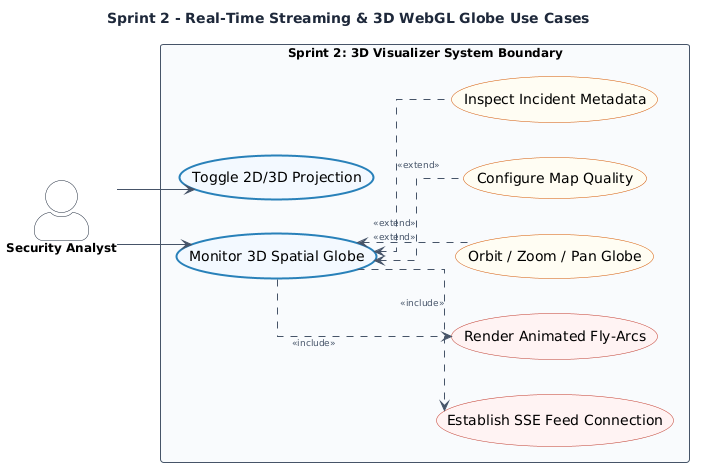
\includegraphics[width=0.95\textwidth]{assets/s2_usecase.png}
\caption{Sprint 2: Use Case diagram for the 3D map visualizer.}
\label{fig:s2_usecase}
\end{figure}

The functional steps are detailed in Table~\ref{tab:s2_uc_desc}.

\begin{table}[htbp]
\centering
\small
\begin{tabular}{>{\raggedright\arraybackslash}p{2.8cm}>{\raggedright\arraybackslash}p{5.2cm}>{\raggedright\arraybackslash}p{5.2cm}}
\toprule
\textbf{Use Case} & \textbf{Actor/Trigger} & \textbf{Main Workflow} \\
\midrule
Monitor 3D Spatial Globe & Security Analyst / Mounts Page & Connects the client browser to the live `/api/feed` stream. Incoming events are geocoded to 3D vectors and drawn as animated great-circle arcs and pulsating circles. \\
Toggle 2D Projection & Security Analyst / Clicks HUD Button & Triggers a coordinate system interpolation, flattening the Three.js mesh spheres into a flat 2D Mercator layout. \\
\bottomrule
\end{tabular}
\caption{Sprint 2: Use Case descriptions.}
\label{tab:s2_uc_desc}
\end{table}

\subsection{Sprint Conception: Trigonometric Geocoding and Arc Interpolation}
Building a high-performance 3D visual mapping environment requires a solid mathematical foundation. To bridge the gap between geographical databases (which express threat locations using standard Latitude/Longitude coordinate systems) and WebGL canvases (which require 3D spatial vector arrays), we designed custom geocoding and curve-generation pipelines.

\subsubsection{Spatial Projection Mathematics (Latitude/Longitude to Vector3)}
To project geolocated coordinates onto the procedural Three.js sphere, the system translates geographic coordinates (standard latitude and longitude values in degrees) into three-dimensional Cartesian vector coordinates. This mapping operates within a coordinate system relative to a sphere of a predefined radius (typically set to a base unit of 1.0).

First, the geographic angles in degrees are mathematically scaled into radians. To ensure the rendered map projection aligns perfectly with the WebGL screen orientation, the longitude is offset by 180 degrees before scaling, and the latitude is directly converted. The system then computes the Cartesian coordinates. The horizontal coordinate (X-axis) is defined as the negative product of the sphere radius, the cosine of the radian latitude, and the cosine of the radian longitude. The vertical coordinate (Y-axis) is defined as the product of the sphere radius and the sine of the radian latitude. Finally, the depth coordinate (Z-axis) is defined as the product of the sphere radius, the cosine of the radian latitude, and the sine of the radian longitude.

The inclusion of the negative sign on the horizontal projection (X-axis) is a critical requirement of the WebGL rendering context. Three.js utilizes a right-handed coordinate system where the positive Z-axis points directly outward from the screen, the positive Y-axis points upwards, and the positive X-axis points rightwards. Omitting this directional inversion would cause the geocoded map coordinates to mirror horizontally, placing geographical boundaries in the incorrect hemispheres.

\subsubsection{Trigonometric Derivation of Spherical Linear Interpolation (SLERP)}
To render an attack arc flying out from a source coordinates vector to a destination coordinates vector across the sphere surface, a simple linear interpolation of coordinates is geometrically incorrect. A linear interpolation (LERP) would cut straight through the three-dimensional volume of the sphere, resulting in a straight line that sinks directly beneath the curved surface mesh of the Earth.

To ensure that the attack trail flies gracefully along the curved surface of the globe, the system utilizes Spherical Linear Interpolation (SLERP). The algorithm first calculates the angular separation between the two unit position vectors (the source vector and the destination vector). This is achieved by taking the vector dot product of the two coordinates, which represents the cosine of the separation angle.

Using this angular separation, the intermediate coordinates are interpolated along the curved surface for any progress state (ranging from zero percent at the start to one hundred percent at the destination). The algorithm scales each of the two terminal vectors using sine-based ratios of the progress state and the total angular separation. This specific sine-based weighting ensures a constant angular velocity across the entire flight path. As a result, the particle trails move at a perfectly uniform speed, avoiding unrealistic accelerations or deceleration spikes near the starting or ending coordinates.

\subsubsection{Parametric Quadratic Bezier Fly-Arcs}
While spherical linear interpolation keeps paths aligned to the sphere's surface, rendering multiple overlapping tracks directly on the globe makes visual analysis difficult. To represent attack vectors as elevated volumetric fibers, the arcs are designed to rise radially outward, reaching their peak altitude exactly at the midpoint of their flight trajectory:
\begin{enumerate}
    \item The system first computes a surface midpoint coordinates vector. This is done by performing a spherical linear interpolation between the source and destination vectors at exactly fifty percent of the flight progress.
    \item An elevated control point vector is then projected radially outward from the center of the sphere. This is achieved by scaling the surface midpoint vector by an elevation multiplier. This multiplier is calculated by adding a base scale factor to the product of a dynamic arc height scalar coefficient (typically set between 0.25 and 0.45) and the angular distance between the source and destination vectors. This dynamic scaling guarantees that long-distance intercontinental attacks arch significantly higher into space, while local regional queries remain low and close to the surface, visually sorting the severity and scope of threat streams.
    \item These three coordinate vectors (the source vector, the elevated control vector, and the destination vector) are passed to the Three.js quadratic Bezier curve constructor. The resulting curve is evaluated parametrically using quadratic Bernstein polynomials to generate a smooth, continuous path. This path starts at the origin coordinates, reaches its maximum radial height in outer space at the midpoint, and sweeps down to the target coordinates, providing a beautiful neon volumetric path.
\end{enumerate}

\subsubsection{UML Sequence Diagram}
The real-time streaming pipeline from scraper broadcasts to frontend Zustand store accumulation and WebGL rendering cycles is traced in Figure~\ref{fig:s2_sequence}.

\begin{figure}[htbp]
\centering
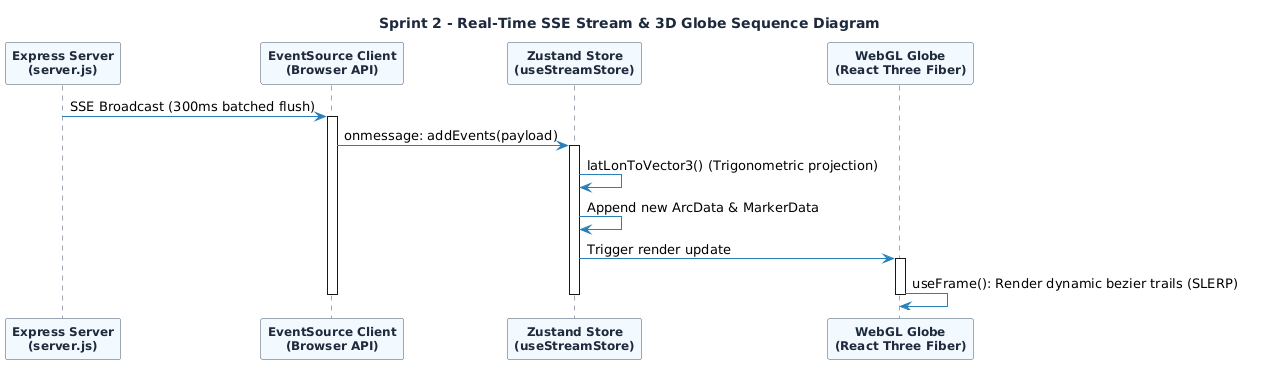
\includegraphics[width=0.95\textwidth]{assets/s2_sequence.png}
\caption{Sprint 2: Sequence diagram of real-time streaming and WebGL rendering.}
\label{fig:s2_sequence}
\end{figure}

---

\subsection{Sprint Realization: Shaders, Shards, and WebGL Globe}

\subsubsection{Server-Sent Events (SSE) Broadcast Engine}
Rather than using heavy WebSockets, we built an optimized SSE route \texttt{GET /api/feed} in \texttt{backend/server.js}:
\begin{itemize}
    \item Sets the required streaming headers: \texttt{Content-Type} (set to \texttt{text/}\allowbreak\texttt{event-stream}), \texttt{Cache-Control} (set to \texttt{no-cache}), and \texttt{Connection} (set to \texttt{keep-alive}).
    \item Incoming scrapers immediately queue threat events into a memory array.
    \item The server runs a \textbf{300ms flush interval scheduler}, consolidating all queued events into a single payload array and writing it to connected clients. This avoids browser rendering lockups from rapid single-event updates.
    \item A \textbf{30-second ping heartbeat} is emitted to keep connections open through proxies.
\end{itemize}

\subsubsection{3D Earth Shader Realization}
Our primary globe mesh in \texttt{globe/Earth.tsx} implements a highly performant, custom-shaded sphere:
\begin{itemize}
    \item \textbf{Custom GLSL Shaders:} To create a premium visual experience, the globe mesh avoids standard flat image textures. Instead, we wrote custom WebGL vertex and fragment shaders using OpenGL Shading Language (GLSL). The vertex shader passes surface normals to the fragment shader, which computes a real-time \textbf{Fresnel atmospheric glow} based on the relationship between the surface normal vector and the camera's line-of-sight view vector. Specifically, the shader calculates the vector dot product of the surface normal and the camera view direction, restricts this value to a non-negative range, subtracts it from a maximum intensity unit, and raises the result to a power falloff factor (typically set to a factor of 4.0). This creates a high-fidelity glowing border around the outer silhouette of the globe that fades smoothly towards the center.
    
    To illustrate this shader logic, Table~\ref{tab:glow_shader_vars} outlines the shader attributes and parameters passed between the rendering passes, with the complete source code detailed in Appendix H.1:

    \begin{table}[htbp]
    \centering
    \small
    \begin{tabular}{lll}
    \toprule
    \textbf{Variable Name} & \textbf{GLSL Type} & \textbf{Role / Computational Purpose} \\
    \midrule
    \texttt{vNormal} & \texttt{varying vec3} & Surface normal vector passed from vertex to fragment shader \\
    \texttt{normalMatrix} & \texttt{uniform mat3} & Standard WebGL transformation matrix mapping normals \\
    \texttt{mvPosition} & \texttt{vec4} & Model-View matrix mapping physical coordinates on sphere \\
    \texttt{dotProd} & \texttt{float} & Dot product measuring normal cosine angle relative to camera \\
    \texttt{intensity} & \texttt{float} & Power-scaled intensity falloff function for Fresnel scattering \\
    \texttt{atmosphericColor} & \texttt{vec3} & Neon Cyberblue color vector (\texttt{0.23, 0.51, 0.96}) \\
    \texttt{gl\_FragColor} & \texttt{vec4} & Output pixel color vector containing transparency blending \\
    \bottomrule
    \end{tabular}
    \caption{Atmospheric Glow Shader Parameters and Interpolated Variables.}
    \label{tab:glow_shader_vars}
    \end{table}
    
    \item \textbf{TopoJSON Country Outlines:} Loads a lightweight TopoJSON land coordinate file (\texttt{land-110m.json}) and projects the land boundaries as vector lines.
    \item \textbf{Neon Glow Borders:} Renders country borders using \textbf{5 overlapping vector line layers} at microscopic scale increases (from $R=1.002$ to $R=1.010$) with decreasing opacities, creating a beautiful neon outline glow effect without needing heavy blur shaders.
    \item \textbf{Post-Processing Bloom:} Wraps the R3F \texttt{<Canvas>} in \texttt{<EffectComposer>}, using a high-fidelity \texttt{<Bloom>} shader (luminanceThreshold 0.15, intensity 0.8) to make severity-colored attack arcs glow like neon light fibers.
\end{itemize}

---

\section{Conclusion}
This chapter detailed the completion of our first main release. By combining a parallel harvester backend with geocoders and establishing the 300ms SSE broadcast channel, we successfully rendered the 3D procedural WebGL threat globe at 60fps, displaying active threat events as volumetric glowing bezier arcs. We proceed to Chapter 4 to document the second release, detailing the analytical STIX 2.1 graph, historical browser, and performance guardrails.
